%
% Norbert Preining
% Article presented on the 5th GuITmeeting, Pisa 18 October 2008
% Übersetzung für DTK
%
% Copyright 2008, 2009 Norbert Preining
% You can redistribute and/or modify this document under the terms of the 
% GNU General Public License as published by the Free Software Foundation; 
% either version 2 of the License, or (at your option) any later version.
%

\newcommand{\tl}{\TeX~Live}
\title{\tl~2008 und der \TeX\ Live Manager%
  \thanks{
	  Dieser Artikel ist eine erweiterte und auf den neusten Stand
  	  gebrachte Version eines ursprünglich am GuIT\ Conference 2008 in 
	  Pisa präsentierten und in Ars\TeX nica, Issue~6 veröffentlichten
	  Artikels}}

\author{Norbert Preining}
\address{Norbert}{Preining}{Technische Universität Wien\\
	%Wiedner Hauptstr.\ 10\\
	%1040 Wien, Austria
}
%\netaddress{preining@logic.at}

\maketitle

\lstset{frame=lines,basicstyle=\small\ttfamily,prebreak={\Righttorque},
  postbreak={\Lefttorque},columns=flexible,breaklines}
\DefineShortVerb{\|}

\newcommand{\tlmgr}{\TeX~Live Manager}

\newcommand{\tlpsrc}{\texttt{tlpsrc}}
\newcommand{\tlpsrcs}{\tlpsrc{}s}
\newcommand{\tlpobj}{\texttt{tlpobj}}
\newcommand{\tlpobjs}{\tlpobj{}s}
\newcommand{\tlpdb}{\texttt{tlpdb}}
\newcommand{\tlpdbs}{\tlpdb{}s}
\newcommand{\pl}{Perl}
\newcommand{\gs}{Ghostscript}
\newcommand{\tlu}{\texttt{texlua}}
\newcommand{\kpse}{Kpathsea}
\newcommand{\XeTeX}{Xe\TeX}
\newcommand{\acro}[1]{\textsc{\MakeLowercase{#1}}}
\newcommand{\ctan}{\acro{CTAN}}
\newcommand{\cmd}[1]{\textsf{#1}}
\newcommand{\button}[1]{\textsf{#1}}
\newcommand{\var}[1]{\textsl{#1}}


\begin{abstract}
Die Release von \tl~2008 vor bald einem Jahr ist die erste Ausgabe
von \tl\ die das neue Programm \tlmgr, kurz tlmgr, mitbringt.

Der \tlmgr\ übernimmt nicht nur einige der Aufgaben von texconfig
(welches niemals für Windows verfügbar war), sondern bereichert die
\tl\ Welt um viele neue Möglichkeiten, darunter die wohl am längsten
gewünschte Fähigkeit zu laufenden Updates.

Der vorliegende Artikel präsentiert das neue \tl\ Installationsprogramm, den
\tlmgr, und beschreibt einige andere Neuigkeiten in \tl~2008.
\end{abstract}


\tableofcontents

\section*{Wichtiger Hinweis}

Dieser Artikel beschreibt den Status des \tlmgr\ wie er im April~2009
verteilt wird, und nicht die Version die auf \acro{DVD} vorhanden ist.
Letztere funktioniert gut für lokale Konfigurationsänderungen
(warum wir das Programm auch auslieferten), aber der Updatemechanismus
übers Internet ist nicht hinlänglich robust. Benutzer der \acro{DVD}
Version sollten zuerst den \tlmgr\ auf den neuesten Stand bringen.

\section{Einführung}
\label{sec:intro}

Nach mehr als einem Jahr der Entwicklung wurde \tl~2008 mit einer
völlig neuen Infrastruktur freigegeben \citep{at:2007-4-069-preining}.
Der Ausgangspunkt dieser Überarbeitung waren zuerst nur notwendige
Vereinfachungen um die Arbeit der Entwickler (etwas) einfacher und das
System aufgrund der Elimination von doppelter Informationen zu
vereinfachen.

Die erste Änderung die für normale Benutzer sichtbar wurde war die
Vereinheitlichung des Installationsprogramms, so dass nun alle
unterstützten Plattformen nun den gleichen Installer verwenden.
Weiters erhielt das Installationsprogramm eine graphische Oberfläche
die ebenfalls einheitlich über alle Plattformen ist. Auf Unix ist die
einzige Voraussetzungen des Installationsprogramms eine Perlinstallation,
und für das graphische Frontend zusätzlich das Vorhandensein von Perl/Tk.
Auf Windows wird eine minimale Perlinstallation mit allen notwendigen
Modulen mitgeliefert, so dass keine weiteren Voraussetzungen gegeben
sind.

Der erste Teil dieses Artikels wird einen Überblick über das 
neue Installationsprogramm geben.

Die zweite für Benutzer sichtbare Änderung ist das neue Programm \tlmgr,
oder kurz tlmgr. Es konfiguriert eine vorhandene \tl\ Installation, sowohl
was Pakete als auch was Optionen und Einstellungen angeht. Es erlaubt neben
vieler Aufgaben die ursprünglich von |texconfig| ausgeführt wurde auch die
Installation von zusätzlichen Paketen, das Update und das Entfernen von 
vorhandenen Paketen, die Erstellung von Backups, die Suche nach und das
Auflisten von Paketen.

\section{Das neue Installationsprogramm}
\label{sec:installer}

Die Erstellung eines neuen \tl\ Installationsprogramms wurde durch das
Umschreiben der Infrastruktur bedingt \citep{at:2007-4-069-preining}. 
Für den Benutzer der \tl\ installiert ergeben sich nur einige Änderungen
im Aussehen, aber dahinter stehen einige wichtige Änderungen, im speziellen:
\begin{itemize}
\item Installationen von \tl\ über das Internet wird ermöglicht.
\item Es gibt nur mehr ein (1) Installationsprogramm, das entweder im 
  Textmodus arbeitet und dabei das frühere Shellskript |install-tl.sh|
  emuliert, oder im \acro{GUI} Modus.
\item Die Installation auf Windowssystemen ist viel näher an der Installation
  auf Unix-Systemen.
\end{itemize}

\subsection{Installation von  \tl\ über das Internet}

Wer die \tl\ \acro{DVD} verwendet kann das Installationsprogramm wie 
üblich direkt von der \acro{DVD} starten. Auf Windows startet dabei
das Installationsprogramm automatisch im graphischen Modus (siehe weiter 
unten), auf Unix-Systemen hingegen im Textmodus.

Ebenfalls ist ein Installationspaket \citep{inst:package} verfügbar
das nur die notwendigen Dateien für eine Installation über das
Internet enthält. Normalerweise wird dabei automatisch ein vom 
|http://mirror.ctan.org| Service ausgewählter Spiegelserver von \ctan\
verwendet (siehe |http://tug.org/ctan.html#sites|).

Dabei werden für die Netzwerkinstallation zwei Pakete zur Verfügung
gestellt. Von |install-tl-unx.tar.gz| unterstützt nur Unix-Systeme,
während |install-tl.zip| zusätzlich auch die notwendige Teilmenge
von Perl für Windows mitbringt. Letzteres funktioniert auf allen
unterstützten Plattformen. Der einzige Grund für die Existenz der
separaten Pakete ist die signifikant kleinere Größe des Installationspaketes
für Unix.

Die voreingestellte Installationsquelle kann durch die Angabe der 
Kommandozeilenoption |-location| beliebig geändert werden.

\subsection{Der Textmodus des Installers}

Wenn Sie \tl\ in den letzten Jahren installiert haben werden Sie keine
großen Änderungen im Textmodus des Installationsprogramms erkennen
((siehe Abb.~\ref{fig:text_main_menu}). Wir haben versucht so nahe wie
möglich am Installationsprogramm der vorherigen Ausgaben zu halten.
Eine neue Option kann am unteren Ende des Menüs gefunden werden:
\emph{set up for running from DVD}. Das ist woher das \emph{Live} in \tl\
kommt: Es erstellt nur eine absolut minimale Umgebung auf dem lokalen
Computer, während alle Eingabedateien und Programme direkt von der
\acro{DVD} verbleiben.

Wie in den vorigen Jahren ist das Installationsprogramm nur in Englisch
verfügbar, während der Graphikmodus jetzt diverse Übersetzungen mitbringt.

\begin{figure}[htp!]
  \centering
  \resizebox{0.8\columnwidth}{!}{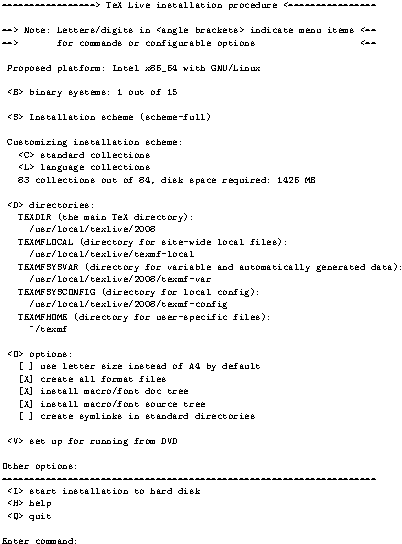
\includegraphics{install08text-crop}}
  \caption{Hauptmenü des Installers im Textmodus}
  \label{fig:text_main_menu}
\end{figure}

\subsection{Der Grafikmodus des Installers}

Der graphische Modus des Installationsprogramms hat fast die gleiche
Funktionalität wie der Textmodus, nur die Option der \emph{Live} Installation
fehlt. Der Grafikmodus ist in Perl/Tk programmiert und sollte auf allen
unterstützten Plattformen laufen (wobei auf Unix Perl/Tk installiert
sein muss).

\begin{figure}[ht!]
  \centering
  \resizebox{0.8\columnwidth}{!}{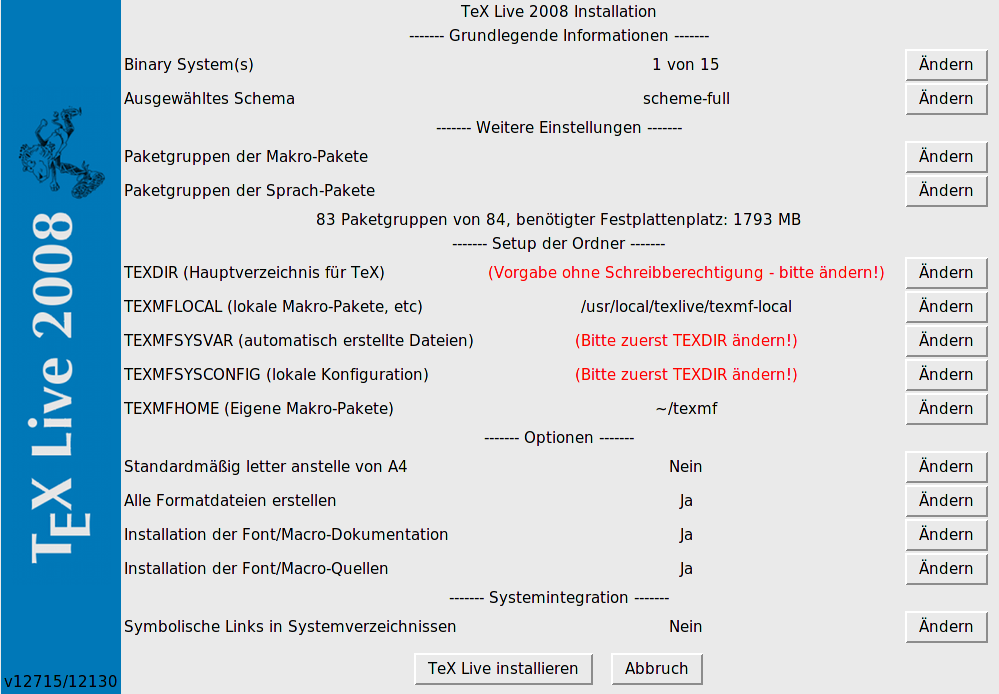
\includegraphics{gui-installer-de.png}}
  \caption{Hauptfenster des graphischen Installers}
  \label{fig:gui_main_menu}
\end{figure}

Abbildung~\ref{fig:gui_main_menu} zeigt das Hauptfenster, dass sehr
an den Textmodus erinnern soll. Wie im Textmodus erlaubt es die zu
installierenden Systeme zu ändern (Abb.~\ref{fig:gui_systems}), ein
Schema auszuwählen (Abb.~\ref{fig:gui_scheme}), wobei ein Schema
eine vordefiniert Auswahl an Paketgruppen ist. Weiters können 
die einzelnen Paketgruppen selber bearbeitet werden, sowie die
Verfügbarkeit von Sprachpaketen und Dokumentation in diversen Sprachen
(Abb.~\ref{fig:gui_coll} und~\ref{fig:gui_lang}). Dann kann der
Installationsordner und verwandte Ordner selektiert werden und 
diverse Optionen an- oder abgewählt werden. All dies sind Funktionalität
wie sie vom Installationsprogramm der letzten Jahre zur Verfügung 
gestellt wurden.

\begin{figure}[ht!]
  \centering
  \resizebox{0.3\columnwidth}{!}{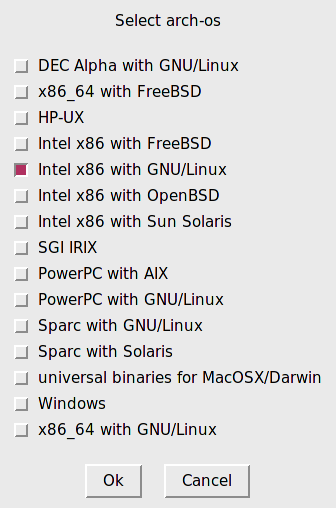
\includegraphics{gui-systems.png}}
  \caption{Auswahlfenster für Binärsysteme}
  \label{fig:gui_systems}
\end{figure}

\begin{figure}[ht!]
  \centering
  \resizebox{0.8\columnwidth}{!}{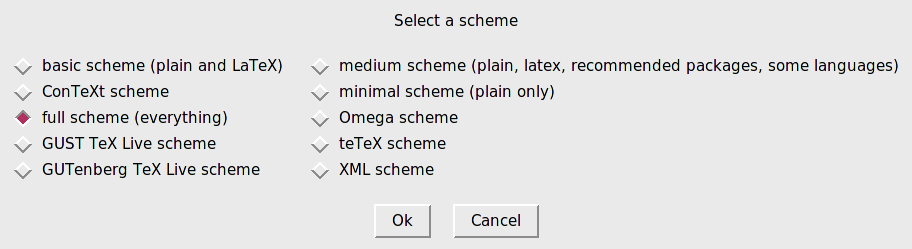
\includegraphics{gui-scheme.png}}
  \caption{Auswahlfenster für Schemata}
  \label{fig:gui_scheme}
\end{figure}

\begin{figure}[ht!]
  \centering
  \resizebox{0.8\columnwidth}{!}{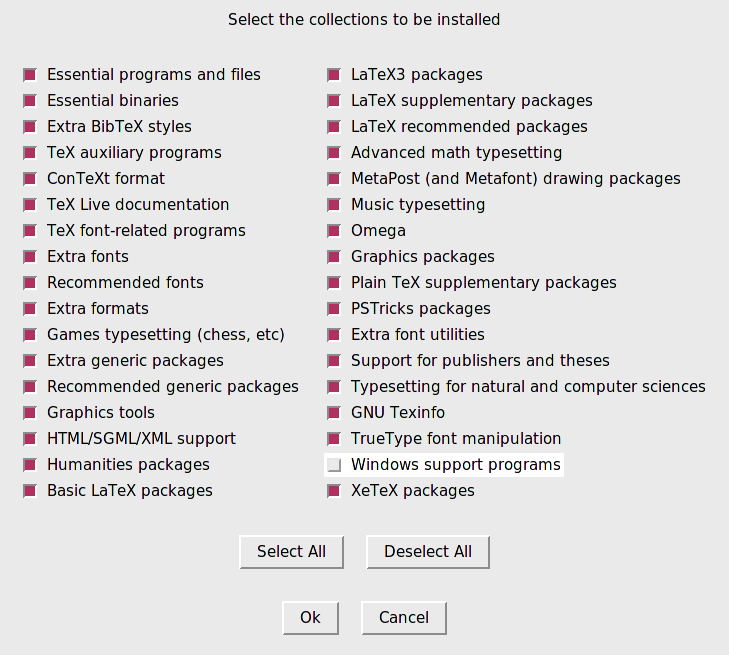
\includegraphics{gui-collections.png}}
  \caption{Auswahlfenster für Paketgruppen}
  \label{fig:gui_coll}
\end{figure}

\begin{figure}[ht!]
  \centering
  \resizebox{0.8\columnwidth}{!}{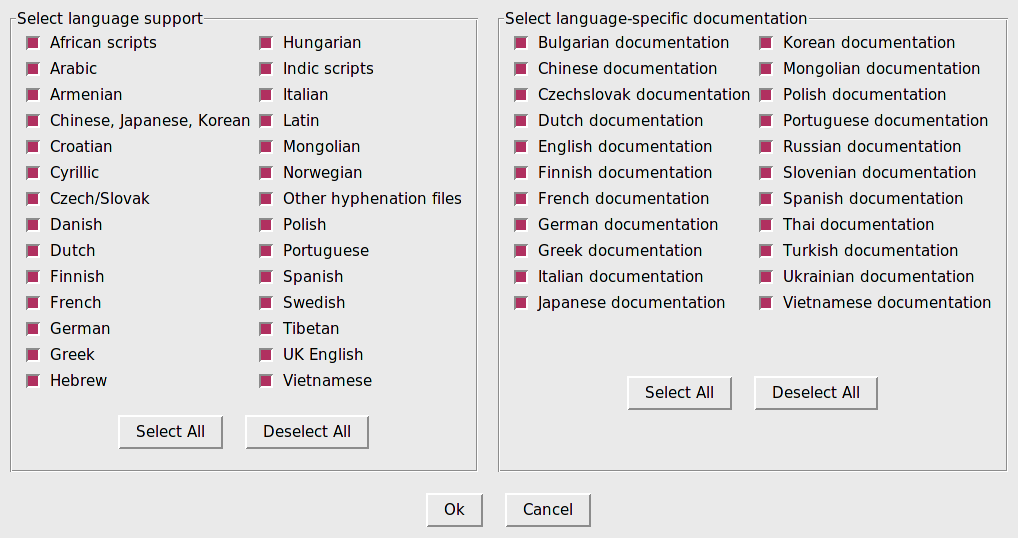
\includegraphics{gui-lang.png}}
  \caption{Auswahlfenster für Sprachpakete}
  \label{fig:gui_lang}
\end{figure}

Sobald die Installation gestartet wird erscheint ein Fenster in dem
der Fortschritt der zu installierenden Pakete angezeigt wird, zusammen mit
Abschätzung der Restzeit und einem Fortschrittsbalken
(Abb.~\ref{fig:gui_progress}).

\begin{figure}[ht!]
  \centering
  \resizebox{0.8\columnwidth}{!}{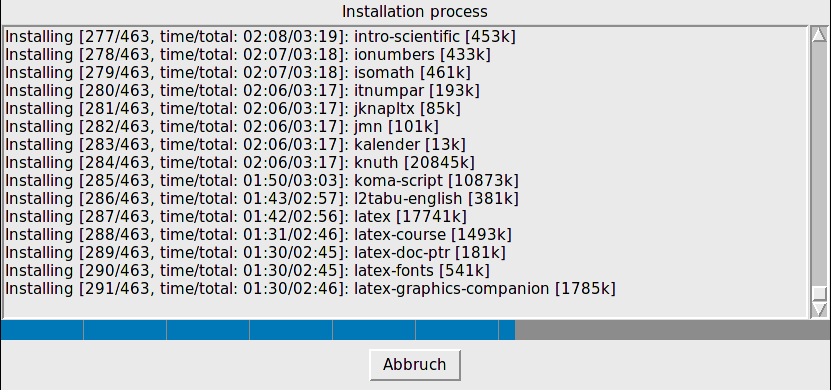
\includegraphics{gui-progress.png}}
  \caption{Fortschrittsfenster}
  \label{fig:gui_progress}
\end{figure}

Sowohl im Textmodus als auch im Graphikmodus des Installationsprogramms
wird eine Logdatei |install-tl.log| mit weiteren Informationen im
im Installationsverzeichnis erstellt. (Bei Fehlerberichten bitte diese
Datei mitschicken!)

\subsection{Windows und Unix rücken näher}

\tl\ 2008 unterstützt nur mehr Windows~2000 und neuere Versionen
(nicht mehr Windows~98), wodurch wir die Notwendigkeit der Spezialbehandlung
von Windows weitgehend reduzieren.

Auf den unterstützten Windows Systemen haben Benutzer ein \emph{echtes}
Heimverzeichnis, nämlich verb+%USERPROFILE%+, das normalerweise
\verb+Dokumente und Einstellungen\+\textit{username} ist.

Dies schlägt sich nun in der Tilde-Erweiterung von \kpse\ nieder:
\verb+~/texmf+ wird auf Windows zu \verb+%USERPROFILE%\texmf+
erweitert, und zu \verb+$HOME/texmf+ auf Unixsystemen.

Wie bisher unter Unix ist es nun auch unter Windows möglich zwischen
systemweiten Einstellungen und Benutzerspezifischen Einstellungen
zu unterscheiden. Weiters gibt es keinen Grund mehr für Windows
verschiedene \texttt{texmf} Bäume zu haben, oder einige Skripts
wie \texttt{fmtutil-sys} und \texttt{updmap-sys} auf Windows nicht
bereitzustellen. Schlussendlich gibt es nun auch eine einzige
\texttt{texmf.cnf} Datei für alle Plattformen.


%
%
%
\section{Der \tlmgr}

Der \tlmgr\ stellt eine Vielzahl an Optionen und Befehlen zur Verfügung, von
denen alle (zum derzeitigen Zeitpunkt implementierten) hier vorgestellt
werden, einige nur sehr kurz, einige detaillierter. Dabei muss man beachten
dass die Entwicklung permanent weitergeht und neue Fähigkeiten laufend
hinzugefügt werden.

\subsection{Die \tl\ Datenbank}

Zu allererst ist es notwendig zu verstehen wo alle Informationen über
installierte Pakete und Optionen gespeichert werden. Dies ist die
\tl\ Datenbank, welche normalerweise in \path{ROOT/tlpkg/texlive.tlpdb}
gefunden werden kann (wobei |ROOT| der Installationsfolder ist).
Diese Datenbank -- eine einfache, jedoch strukturierte Textdatei --
enthält die Liste der installierten Pakete, zu jedem Paket die Liste
der installierten Dateien, und sammelt zusätzlich alle
Konfigurationsoptionen wie die Installationsquelle oder die bei der
Installation angewählten Optionen.

Die meisten der Aktionen von tlmgr laden die lokale Datenbank, und viele
Aktionen laden zusätzlich die \emph{entfernte} Datenbank, also die
von der installiert wird: Wenn Sie zum Beispiel ein Paket installieren
wollen wird die Datenbank der Installationsquelle geladen und überprüft
ob das Paket dort vorhanden ist.

Wobei mit \emph{entfernte} Datenbank nicht unbedingt eine entfernter
Server gemeint ist. Wenn Sie von der \acro{DVD} installiert haben so
wird die Installationsquelle die \acro{DVD} sein, und tlmgr wird diese
Datenbank lande sobald es notwendig ist.

\subsection{Allgemeine Syntax von tlmgr}

Jeder Aufruf von tlmgr sieht wie folgt aus:
\begin{center}
  \Verb+tlmgr [opt]... action [opt]... [arg]...+
\end{center}
Die ersten Optionen vor der Aktion |action| bestimmen einige allgemeine
Einstellungen von tlmgr, während der zweite Satz von Optionen nach der
Aktion spezifisch für die Aktion sind.

Die derzeitige Version unterstützt -- im Gegensatz zu früheren Versionen --
die Vermischung all dieser Optionen. Damit ist es im Prinzip egal was
wo wann kommt. Dennoch werden die Optionen und Aktionen in dieser
Art präsentiert um die Darstellung zu erleichtern.

Der erste Satz kann die folgenden Optionen enthalten:
\begin{itemize}
\item |--location| \var{loc} gibt die Installationsquelle an von der
  Pakete installiert und erneuert werden. Diese Option überschreibt die
  voreingestellte Installationsquelle in der \tl\ Datenbank (\acro{TLPDB}).
\item |--gui| startet die graphische Oberfläche des tlmgr. Diese
  Oberfläche unterstützt nicht den vollen Funktionsumfang der Kommandozeile,
  sehr wohl aber die wichtigsten und häufigsten.
  Der Unterschied zwischen der |--gui| Option und der |gui| Aktion (siehe
  weiter unten) ist dass wenn Sie die Option |--gui| geben und eine Aktion,
  dann versucht tlmgr sofort den entsprechenden Bildschirm der graphischen
  Oberfläche zu laden.
\item |--gui-lang| \var{ll} selektiert die Sprache der graphischen
  Oberfläche. Normalerweise versucht tlmgr die korrekte Sprache aus
  den Umgebungseinstellungen abzuleiten (unter Windows wird die
  Registry befragt, unter Unix |LC_MESSAGES|). Sollte dies fehlen
  erlaubt diese Option eine Sprache auszuwählen.
\item |--machine-readable| Anstelle der normalen Ausgabe die für einen
  menschlichen Benutzer gedacht ist, schaltet diese Option zu einer
  leichter von Programmen parsebaren Ausgabe um. Details können in der
  manpage \citep{tlmgr-manpage} gefunden werden.
\item |--package-logfile| \var{file} tlmgr führt eine Logdatei für alle
  Aktionen die Pakete betreffen (Installation, Entfernen, Update, etc).
  Diese Logdatei ist normalerweise |TEXMFSYSVAR/web2c/tlmgr.log|, diese
  Option erlaubt eine andere Datei anzugeben.
\item |--pause| lässt tlmgr vor Terminierung auf eine Eingabe des Users
  warten. Dies kann auf Windows nützlich sein um das vorschnelle
  Verschwinden des Kommandofensters zu verhindern.
\end{itemize}

Weiters werden diverse Standardoptionen unterstützt: |--help| (oder
|-h|) gibt die manpage aus, |-q| unterdrückt rein informative
Ausgaben, |-v| (verbose) um den Grad der Gesprächigkeit von tlmgr, sprich
den Debuglevel, einzustellen. Mit |--version| gibt tlmgr die Version
des installierten \tl\ Systems als auch die Versionsnummer von tlmgr selbst
aus.

\subsection{Die Aktionen}


Die derzeitige Liste der Aktionen ist:
|help|, |version|, |gui|, |install|, |update|, |backup|, |restore|,
|remove|, |option|, |symlinks|, |paper|, |arch|, |search|, |show|, |list|,
|check|, |uninstall|, |generate|.

\paragraph{Die allgemeinen Aktionen}

\begin{itemize}
\item |search [|\var{option}|...] |\var{what} Ohne zusätzliche Optionen
  wird in der Liste der lokal installierten Pakete in den Paketnamen und
  -beschreibungen nach |what| gesucht. Wird die Option |--global| gegeben,
  so wird die entfernt Datenbank auch durchsucht (sprich auch alle nicht
  installierten Pakete). Wird die Option |--file| gegeben dann werden
  nicht die Paketnamen und -beschreibungen durchsucht, sondern die 
  installierten Dateinamen.
\item |show |\var{pkg}|...| zeigt detaillierte Informationen über die
  angegebenen Pakete an. Falls alle angegebenen Pakete lokal installiert
  sind wird die entfernte Datenbank nicht befragt.
\item \Verb+list [collections|schemes]+ Ohne jegliche Argumente werden alle
  Pakete die bei der Installationsquelle vorhanden sind aufgelistet, wobei
  bereits installierte ein Präfix von "i " erhalten.
  Mit einem Argument werden entweder nur die Paketgruppen oder die Schemata
  aufgelistet, je nach Argument.
\item \Verb+symlinks [add|remove]+ Fügt symbolische Verweise für die
  Programme, die man pages, und die info Dokumentationen hinzu oder
  entfernt sie in den in der Datenbank eingetragenen Ordnern (siehe weiter
  unten unter |option|).
\item |uninstall| Diese Aktion fragt zuerst noch einmal nach, dann wird
  die gesamte Installation entfernt. Wird die Option |--force| gegeben dann
  wird nicht einmal nachgefragt. 
\item \Verb+check [files|collections|all]+ Führt einen oder alle Tests
  der Installation auf Konsistenz durch. Mit |files| wird überprüft
  ob all in der Datenbank gelisteten Dateien auch im System vorhanden 
  sind. Die Option |--use-svn| benutzt den |svn| Befehl um die 
  vorhandenen Dateien festzustellen.
\item |gui| startet die graphische Oberfläche wie oben erklärt.
\item |version| ist das Gleiche wie  |--version|.
\item |help| ist das Gleiche wie |--help|.
\end{itemize}

\paragraph{Die Konfigurationsaktionen}
\begin{itemize}
\item |option [show]| Zeigt alle in der lokalen Datenbank gespeicherten
  Optionen an.
\item |option |\var{key} |[|\var{value}|]| 
  Ohne \var{value} wird der aktuelle Wert der Konfigurationsoption \var{key}
  angezeigt. Derzeit werden die folgenden |key|s werden derzeit akzeptiert:
  |location| -- voreingestellte Installationsquelle; 
  |formats| -- Formate werden bei Installation/Update neu erstellt;
  |docfiles| -- bei der Installation von Paketen werden auch die
    Dokumentationsdateien installiert. Änderung der Option |docfiles| betrifft
    nicht schon installierte Pakete, sondern nur neue Pakete und 
    Updates;
  |srcfiles| -- bei der Installation von Paketen werden auch die
    Quelldateien installiert;
  |backupdir| -- voreingestellter Ordner für Backups;
  |autobackup| -- Anzahl der Backups die behalten werden sollen (siehe
    weiter unten für Details);
  |sys_bin| -- Ordner in dem symbolische Verweise für Programme 
    durch |symlinks| angelegt werden;
  |sys_man| -- Ordner in dem symbolische Verweise für man pages
    durch |symlinks| angelegt werden;
  |sys_info| -- Ordner in dem symbolische Verweise für info Dokumentationen
    durch |symlinks| angelegt werden.
\item |paper |\var{paper} legt das voreingestellte Papierformat ein, entweder
  |a4| oder |letter|. Ohne \var{paper} werden die aktuellen Papierformate
  für alle unterstützten Programme angezeigt.
\item \var{program} \Verb+paper [help|+\var{paper}|]|
  Diese Variante erlaubt es verschiedene voreingestellte Papierformate
  für die unterstützten Programme einstellen. \var{program} kann 
  dabei eines aus |xdvi|, |dvips|, |pdftex|, |dvipdfm|,
  |dvipdfmx|, |context| sein. 
  Ohne zusätzlichem Argument wird das aktuelle Papierformat für \var{program}
  angezeigt. Mit |help| werden alle unterstützten Papierformate für 
  das jeweilige Programm angezeigt. Mit der Angabe eines Papierformates
  wird das Programm für dieses Format umkonfiguriert.
\item |generate |\var{what} Diese Aktion erstellt ein oder mehrere
  Konfigurationsdateien wie folgt beschrieben:
  
  Wird für \var{what} der Wert |language.dat| angegeben, dann wird 
  die Datei |language.dat| welche die Trennmuster die in \LaTeX-basierende
  Formate geladen werden erstellt.
  Mit |language.def| wird ebendiese Datei erstellt, die die Trennmuster
  die in |etex|-basierende Formate geladen werden festlegt.
  Wird nur |language| für \var{what} angegeben so werden beide Dateien
  erstellt.
  
  Wird |fmtutil| für \var{what} angegeben so wird die Datei |fmtutil.cnf|
  neu erstellt, die die Definitionen aller zu erstellenden Formate
  enthält.

  Wird |updmap| für \var{what} angegeben so wird die Datei |updmap.cfg|
  neu erstellt, die alle installierten Schriftarten-map Dateien enthält.

  Für |fmtutil.cnf| und die beiden |language| Dateien ist das neu
  Erstellen normal und sowohl das Installationsprogramm als auch tlmgr
  tun dies regelmäßig.

  Für |updmap.cfg| jedoch ist dies nicht so. Weder das Installationsprogramm
  noch tlmgr verwenden den |generate| Aufrufs, da dieser alle manuell
  aktivierten Schriftarten-map Dateien die mit |updmap-sys --enable|
  aktiviert worden sind, entfernen (z.B.\ für lokal installierte
  kommerzielle Fonts). Nur Eintragungen die in |--localcfg| (siehe weiter 
  unten) eingetragen sind würden erhalten werden.

  Wenn Sie jedoch nur Schriftarten aus \tl\ selbst verwenden, dann
  ist der Aufruf von |generate| ohne negativen Konsequenzen. Wir verwenden
  es um die Datei |updmap.cfg| in unserem Repository zu aktualisieren.

  Sollten die Dateien |language-local.dat|, |language-local.def|,
  |fmtutil-local.cnf|, oder |updmap-local.cfg| vorhanden sein unter
  \path{TEXMFLOCAL} in den entsprechenden Ordnern, dann wird deren
  Inhalt als letztes in die erstellten Dateien hineinkopiert.
\end{itemize}


\paragraph{Die Paketaktionen}
\begin{itemize}
\item |install| \var{pkg}\ldots\ installiert die angegebenen Pakete.
  Normalerweise werden alle Pakete von denen ein angegebenes Paket
  abhängt auch mitinstalliert. Dies kann mit der Option |--no-depends|
  unterdrückt werden. Weiters gibt es noch |--no-depends-at-all|
  was tlmgr zusätzlich die eng verknüpften Pakete mit architekturspezifischen
  Paketen vergessen lässt; zum Beispiel |bin-bibtex| und
  |bin-bibtex.i386-linux|. Das sollte niemals verwendet werden außer Sie
  wissen sehr genau was Sie tun.
  |--dry-run| simuliert die Installation nur.
\item |update| \var{pkg}\ldots\  bringt die angegebenen Pakete auf den
  neuesten Stand. Zusätzlich, sollte ein der \var{pkg} eine Paketgruppe
  sein, und an der Installationsquelle gibt es die gleiche Paketgruppe
  mit Paketen die nicht installiert sind lokal, so werden diese auch
  installiert. Optionen sind:
  \begin{description}
  \item |--list| Listet nur die Pakete auf die erneuert oder 
    neu installiert werden würden ohne den Update wirklich durchzuführen.
    Es werden zusätzlich die Revisionsnummern der lokalen Pakete und
    der Pakete der Installationsquelle angegeben.
  \item |--all| Bringt alle Pakete die Erneuerungen haben auf den neuesten
    Stand.
  \item |--dry-run| Die Installation wird nur simuliert.
  \item |--backup| und |--backupdir |\var{directory}
    Diese Optionen steuern die Erstellung von Sicherheitskopien der
    Pakete bevor das Upgrade installiert wird.
    Wird weder |--backup| noch |--backupdir| angegeben wird keine
    Sicherheitskopie erstellt. Wird |--backupdir| angegeben und 
    zeigt auf einen beschreibbaren Ordner, wird eine Sicherungskopie
    erstellt. Wird nur |--backup| angegeben wird versucht der in der
    Datenbank vorher mit |option backupdir| festgelegte Ordner für
    Sicherungskopien zu verwenden.
    Werden beide Optionen angegeben dann wird die Sicherungskopie in
    dem angegebenen Ordner erstellt.

    tlmgr erstellt vor jedem Upgrade eine temporäre Sicherungskopie um
    im Fehlerfall automatisch zur letzten installierten Version
    zurückgehen zu können. Diese Optionen hier erlauben die Erstellung
    von persistenten Sicherungskopien.

  \item |--no-depends| Normale Abhängigkeiten werden nicht aufgelöst.
  \item |--no-depends-at-all| Bitte die |install| Aktion weiter oben
    dazu konsultieren.
  \end{description}
\item |remove| \var{pkg}\ldots\ 
  entfernt die angegebenen Pakete. Wird eine Paketgruppe entfernt
  werden auch alle darin gelisteten Pakete entfernt, jedoch keine
  anderen Paketgruppen die darin referenziert sind. 
  Wird ein normales Pakete (keine Paketgruppe) entfernt dann werden
  darin referenzierte Pakete nie entfernt.

  Options:
  \begin{description}
  \item |--no-depends| referenziert Pakete werden nicht entfernt.
  \item |--no-depends-at-all| Bitte die |install| Aktion weiter oben
    dazu konsultieren.
  \item |--force|
    tlmgr überprüft ob ein zu entfernendes Paket oder Paketgruppe
    in irgendeinem anderen Paket oder Paketgruppe referenziert ist. Ist
    dies so wird das Paket oder die Paketgruppe nicht entfernt
    außer man gibt diese Option an.
  \item |--dry-run|
    Das Entfernen der Pakete wird nur simuliert.
  \end{description}
\item |backup| \var{pkg}\ldots\
  Wird die Option |--clean| nicht angegeben, wird von den angegebenen
  Paketen, oder von allen wenn |--all| angegeben ist, eine 
  Sicherungskopie gemacht. Diese Kopien werden in den Ordner der
  entweder durch die Option |--backupdir| angegeben ist, oder durch
  den in der Datenbank festgelegten Ordner bestimmt. Sollten beide
  nicht angegeben sein oder nicht beschreibbar, werden keine 
  Sicherungskopien erstellt.

  Wird |--clean| angegeben dann werden alte Sicherungskopien gelöscht.
  Der Wert der zu erhaltenden Sicherungskopien wird entweder durch
  einen optionalen Parameter zu |--clean=N| angegeben, oder durch den
  in der Datenbank gespeicherte Option |autobackup|.

\item |restore --backupdir |\var{dir} |[|\var{pkg} |[|\var{rev}|]]|\\
  Wird \var{pkg} nicht angegeben (und daher auch kein \var{rev}), dann
  werden alle vorhanden Sicherungskopien für alle Pakete aufgelistet.
 
  Wird \var{pkg} angegeben aber kein \var{rev} dann werden alle 
  vorhandenen Sicherungskopien nach Revisionen für das Paket
  aufgelistet.

  Werden sowohl \var{pkg} als auch \var{rev} angegeben wird die 
  Sicherungskopie des Pakets in der angegebenen Revision installiert.

  Die Option |--backupdir dir| gibt den Ordner an wo nach 
  Sicherungskopien gesucht wird.
  Die Option |--dry-run| wird ebenso unterstützt, wie üblich.
  
\item |arch |\var{operation} \var{arg}\ldots
  Ist \var{operation} gleich |list| so werden alle an der 
  Installationsquelle vorhandenen Architekturen/Plattformen ausgegeben.
  
  Ist \var{operation} gleich |add| so werden die Programme für die 
  angegebenen Architekturen installiert.
  
  Die Option |--dry-run| wird ebenso unterstützt, wie üblich.
\end{itemize}


\subsection{Typische Anwendungsbeispiele des tlmgr}

Im Folgenden werden wir einige typische Anwendungsszenaria des \tlmgr\
vorstellen.

\paragraph{Installation einer neuen Paketgruppe}

Angenommen Sie haben das Schema |scheme-medium| installiert und
realisieren dass die Trennmuster für einige Sprachen die Sie benutzen
fehlen, z.B.\ Norwegisch. Zuerst verwenden Sie tlmgr um nach diesem
Schlüsselwort zu suchen:
\begin{lstlisting}
$ tlmgr search --global norwegian
tlmgr: installation location ...
collection-langnorwegian - Norwegian
hyphen-norwegian - 
\end{lstlisting}
und dann installieren Sie die Paketgruppe:
\begin{lstlisting}
$ tlmgr install collection-langnorwegian
tlmgr: installation location ...
install: collection-langnorwegian
install: hyphen-norwegian
tlmgr: package log updated at .../tlmgr.log
regenerating language.dat
regenerating language.def
\end{lstlisting}
gefolgt von der Ausgabe der Neuerstellung aller Formate die entweder von
|language.dat| oder |language.def| abhängen.
(Falls die |formats| Option auf 0 geändert wurde in der lokalen Datenbank
wird die Neuerstellung übersprungen. Die Voreinstellung ist dass Format
jeweils erneuert werden.)

\paragraph{Suche nach einem Paket}

Sie wollen eine Einladung mit Absätzen in besonderen Formen setzten, aber
Sie wissen nicht welches Paket man da verwenden könnte. Ein Aufruf von
tlmgr hilft:
\begin{lstlisting}
$ tlmgr search paragraph
\end{lstlisting}
zeigt aber keine Ausgabe. Vielleicht ist nichts entsprechendes installiert?
Also versuchen Sie eine Globalsuche:
\lstset{breaklines}
\begin{lstlisting}
$ tlmgr search -global paragraph
tlmgr: installation location ...
 bigfoot - Footnotes for critical editions
 edmargin - Multiple series of endnotes for critical editions
 footmisc - A range of footnote options
 genmpage - Generalization of LaTeX's minipages
 hanging - Hanging paragraphs
 ibycus-babel - Use the Ibycus 4 Greek font with Babel
 insbox - A TeX macro for inserting pictures/boxes into paragraphs
 layouts - Display various elements of a document's layout
 lettrine - Typeset dropped capitals
 lineno - Line numbers on paragraphs
 lipsum - Easy access to the Lorem Ipsum dummy text
 moresize - Allows font sizes up to 35.83pt
 ncctools - A collection of general packages for LaTeX
 paralist - Enumerate and itemize within paragraphs
 picinpar - Insert pictures into paragraphs
 plari - Typesetting stageplay scripts
 seqsplit - Split long sequences of characters in a neutral way
 shapepar - A macro to typeset paragraphs in specific shapes
 vwcol - Variable-width multiple text columns
\end{lstlisting}
und hier ist es, |shapepar| scheint genau zu sein was Sie brauchen. Also
sehen Sie sich genauer an was diese Paket ist:
\begin{lstlisting}
$ tlmgr show shapepar
tlmgr: installation location ...
Package:   shapepar
Category:  Package
ShortDesc: A macro to typeset paragraphs in specific shapes.
LongDesc:  \shapepar is a macro to typeset paragraphs in a specific shape.
...
Installed: No
Collection:collection-latexextra
\end{lstlisting}
Nun, das schaut gut aus. Sie können nun entweder die ganze Paketgruppe
installieren:
\begin{lstlisting}
$ tlmgr install collection-latexextra
\end{lstlisting}
was aber nicht nur |shapepar| sondern eine Unmenge anderer Pakete mitbringt,
oder sie installieren nur dieses eine Paket und hoffen dass keine
anderen Pakete notwendig sind:
\begin{lstlisting}
$ tlmgr install shapepar
tlmgr: installation location ...
install: shapepar
tlmgr: package log updated at .../tlmgr.log
running mktexlsr
...
\end{lstlisting}

Diese Beispiele demonstrieren wie man nicht installierte Pakete findet
und installiert. Die Voreinstellung des Installationsprogrammes ist
jedoch das gesamte \tl\ zu installieren, d.h.\ alles was verfügbar ist
wird auch installiert.

\paragraph{Update der Installation}

Nach der ersten Installation wollen Sie nun die neuesten Versionen der
gesamten Pakete bekommen, doch sicherheitshalber vorher überprüfen
was denn das heißt:
\begin{lstlisting}
$ tlmgr update --list
tlmgr: installation location /mnt/cdrom
Cannot load TeX Live database from /mnt/cdrom at .../tl/2008/bin/i386-linux/tlmgr line 1505, <TMP> line 1982.
\end{lstlisting}
Hmm, das scheint ein Fehler sich eingeschlichen zu haben, tlmgr versucht
noch immer von der \acro{DVD} zu installieren, die Sie schon lange
an einen Freund weitergegeben haben. Da sollte Sie nun zur
Netzwerkinstallationsquelle übergehen, und das gleich für alle weiteren
Aktionen als Voreinstellung speichern. Nur haben Sie schon wieder die
Adresse vergessen! Glücklicherweise kann sich der \tlmgr\ daran erinnern
und Sie brauchen ihm nur sagen dass er |ctan| verwenden soll:
\begin{lstlisting}
$ tlmgr option location ctan
tlmgr: setting default installation location to http://mirror.ctan.org/systems/texlive/tlnet/2008
\end{lstlisting}
Ok, nun schauen wir mal was es so Neues gibt:
\begin{lstlisting}
$ tlmgr update --list
tlmgr: installation location /src/TeX/texlive-svn/Master
bin-texlive: local: 12181, source: 12269
cc-pl: local: 7340, source: 12724
latexmk: local: 12697, source: 12749
mfpic4ode: local: 7340, source: 12734
pkfix-helper: local: 12532, source: 12713
scheme-minimal: local: 10129, source: 12703
texlive.infra: local: 12186, source: 12729
\end{lstlisting}
Da sind ja einige Dinge die ein Update brauchen, tun wir das einmal:
\begin{lstlisting}
$ tlmgr update --all
tlmgr: installation location ...
Updates for tlmgr itself are present.
===========================================
Please update the packages bin-texlive and texlive.infra first, via either
  tlmgr update bin-texlive texlive.infra
or by getting the latest updater for Unix-ish systems:
  http://mirror.ctan.org/systems/texlive/tlnet/2008/update-tlmgr-latest.sh
and/or Windows systems:
  http://mirror.ctan.org/systems/texlive/tlnet/2008/update-tlmgr-latest.exe
Then continue with other updates.
===========================================
.../tl/2008/bin/x86_64-linux/tlmgr: Exiting, please read above warning.
\end{lstlisting}
Ja, dies sollte gemacht werden. \tlmgr\ verweigert die Operation wenn
Updates für tlmgr oder die Infrastrukturpakete zur Verfügung stehen.
Dies garantiert dass Fehler im \tlmgr\ nicht zu lange unbehoben bleiben.
Also tun Sie das:
\begin{lstlisting}
$ tlmgr update bin-texlive texlive.infra
tlmgr: installation location ...
[1/2] update: bin-texlive (12181 -> 12269) ... running post remove action for bin-texlive
running post install action for bin-texlive
done
[2/2] update: texlive.infra (12186 -> 12729) ... running post install action for texlive.infra
done
tlmgr: package log updated at .../tlmgr.log
running mktexlsr
...
\end{lstlisting}
Gut, scheint ja geklappt zu haben. Jetzt probieren wir das mit den 
Updates noch einmal:
\begin{lstlisting}
$ tlmgr update --list
tlmgr: installation location ...
cc-pl: local: 7340, source: 12724
latexmk: local: 12697, source: 12749
mfpic4ode: local: 7340, source: 12734
pkfix-helper: local: 12532, source: 12713
scheme-minimal: local: 10129, source: 12703
\end{lstlisting}
und das tatsächliche Upgrade:
\begin{lstlisting}
$ tlmgr update --all
tlmgr: installation location ...
[1/5] update: cc-pl (7340 -> 12724) ... done
[2/5] update: latexmk (12697 -> 12749) ... done
[3/5] update: mfpic4ode (7340 -> 12734) ... done
[4/5] update: pkfix-helper (12532 -> 12713) ... done
[5/5] update: scheme-minimal (10129 -> 12703) ... done
tlmgr: package log updated at .../tlmgr.log
running mktexlsr ...
running updmap-sys  ...
\end{lstlisting}

\paragraph{Einstellen des Papierformats}

Sie übersiedeln nach Japan und hätten gerne \emph{letter} als
voreingestelltes Papierformat, nichts leichter als das:
\begin{lstlisting}
$ tlmgr paper letter
\end{lstlisting}
und die wichtigsten Programme werden ab nun \emph{letter} Papierformat
verwenden.

\section{Die graphische Oberfläche von tlmgr}

Um die meisten Windows-Benutzer und einige Unix-Benutzer glücklich(er)
zu machen gibt es für tlmgr auch eine graphische Oberfläche, die wie
die des Installationsprogrammes in Perl/Tk geschrieben ist.
Bisher ist jedoch nicht die volle Funktionalität der Kommandozeilenversion
von tlmgr in der graphischen Oberfläche abgebildet.

Die Oberfläche hat mehrere Fenster mit verschiedenen Funktionalitäten:
Installation, Update, Entfernen von Paketen, Entfernen von \tl\ als
Ganzes, Unterstützung verschiedener Architekturen, und Konfiguration.

Die graphische Oberfläche wird mit |tlmgr gui| oder |tlmgr --gui action|
gestartet. Im letzeren Fall versucht tlmgr gleich das Fenster das zur
angegebenen Aktion passt anzuzeigen.

\subsection{Das Installationsfenster}

Das erste Fenster das man normalerweise sieht ist das Installationsfenster
(fig.~\ref{fig:gui:install}).

\begin{figure}[ht!]
  \centering
  \resizebox{0.8\columnwidth}{!}{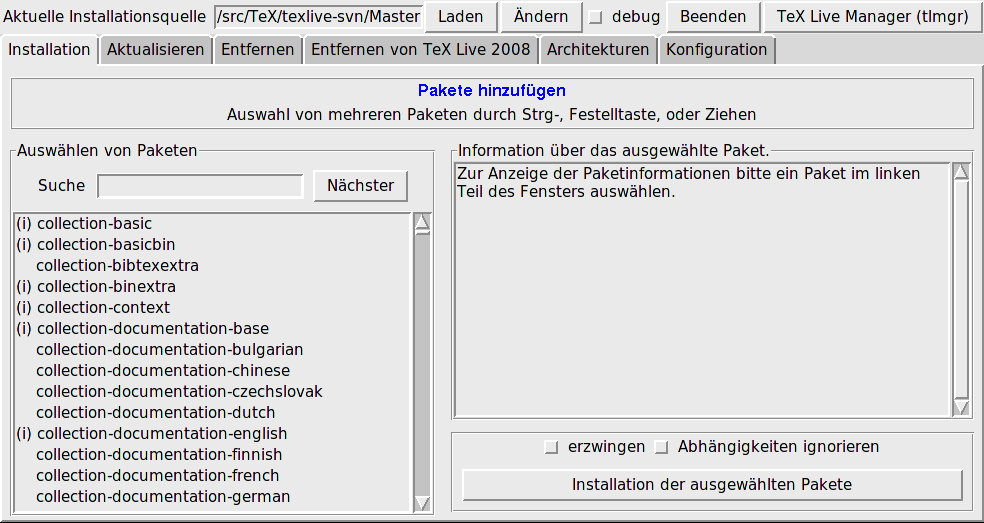
\includegraphics{tlmgrgui-install-de.png}}
  \caption{\tlmgr\ \acro{GUI} Installationsfenster}
  \label{fig:gui:install}
\end{figure}

Am oberen Ende sieht man die aktuelle Installationsquelle, die entweder
über die Kommandozeilenoption |--location| angegeben wurde oder aus 
der Datenbank gelesen wird. Die entfernte Datenbank wird \emph{nicht}
automatisch geladen, Sie müssen die \button{Load} Knopf drücken, oder
den \button{Change} Knopf um vorher eine andere Installationsquelle
anzugeben. 

Darunter sieht man die Liste der an der Installationsquelle verfügbaren
Pakete auf der linken Seite, zuerst die Paketgruppen und Schemata, danach
alle normalen Pakete in alphabetischer Ordnung. Durch Eingabe von Zeichen
in das Eingabefeld neben \button{Suche} hüpft die Selektion sofort zum ersten
passenden Paket. Der Knopf \button{Nächster} erlaubt es zum nächsten
passenden Eintrag zu springen. 

Nachdem ein Paket auf der linken Seite selektiert wurde erscheint die
Kurz- und Langbeschreibung des Paketes im rechten Teil des Fensters.

Darunter gibt es einen Knopf um die selektierten Pakete zu installieren.
Weiters zwei Auswahlschalter die es erlaubt die Installations zu
erzwingen (falls Updates für tlmgr selbst vorhanden sind wird keinerlei
Aktion durchgeführt), und einen Auswahlschalter der es erlaubt Pakete
ohne Abhängigkeiten zu installieren.

\subsection{Das Aktualisierungsfenster}

Der Aktualisierungsfenster ähnelt dem Installationsfenster, mit dem
Unterschied dass nur die Pakete angezeigt werden für die Aktualisierungen
zur Verfügung stehen. Der Aktionsbereich im rechten unteren Eck erlaubt
entweder alle Pakete zu aktualisieren, oder nur die selektierten.
Wieder kann die Aktualisierung erzwungen werden falls neuere Versionen
von tlmgr selbst vorhanden sind.

In Abb.~\ref{fig:gui:update} ist der Aktualisierungsfenster sehen in dem für
einige Pakete Aktualisierungen verfügbar sind.

\begin{figure}[ht!]
  \centering
  \resizebox{0.8\columnwidth}{!}{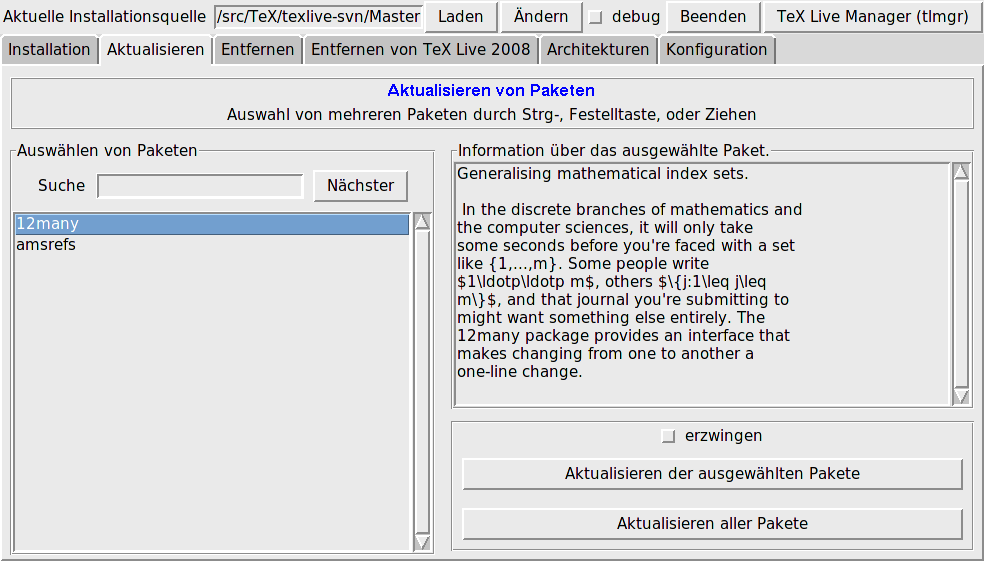
\includegraphics{tlmgrgui-update-de.png}}
  \caption{\tlmgr\ \acro{GUI} Aktualisierungsfenster}
  \label{fig:gui:update}
\end{figure}

\subsection{Das Entfernfenster}

Das Entfernfenster in Abb.~\ref{fig:gui:remove}
ist ebenfalls dem Installationsfenster ähnlich, wobei
die Liste aller installierten Pakete angezeigt werden. Das Aktionsfeld
enthält diesmal einen Knopf um alle selektierten Pakete zu entfernen, und
zwei Auswahlschalter um die Entfernung zu erzwingen (entsprechend
der |--force| Kommandozeilenoption) und Abhängigkeiten zu ignorieren
(entsprechend der |--no-depends| Kommandozeilenoption), 

\begin{figure}[ht!]
  \centering
  \resizebox{0.8\columnwidth}{!}{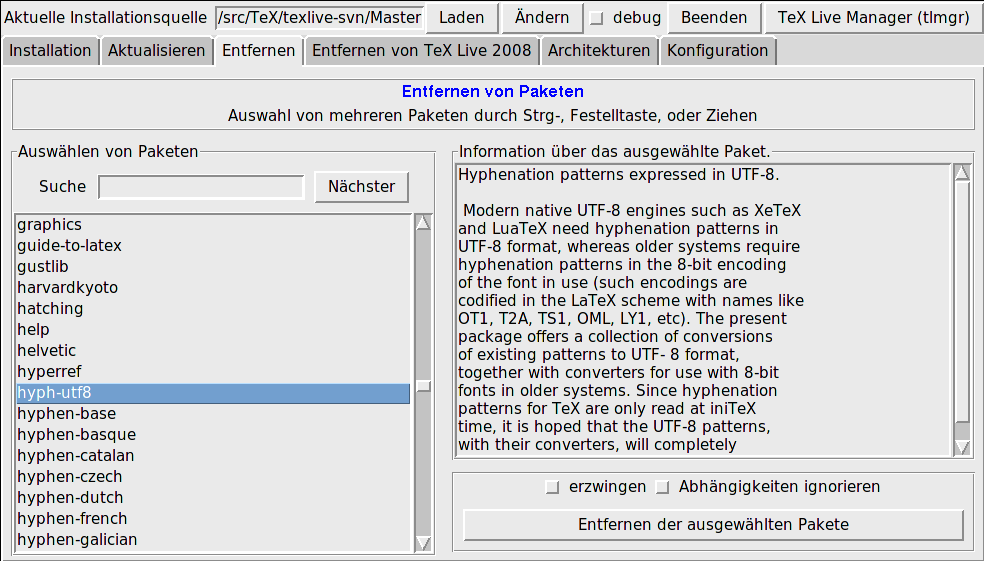
\includegraphics{tlmgrgui-remove-de.png}}
  \caption{\tlmgr\ \acro{GUI} Entfernfenster}
  \label{fig:gui:remove}
\end{figure}

\subsection{Das Deinstallationsfenster}

Dieses Fenster enthält nur einen Knopf der es erlaubt \tl\ vollständig
zu entfernen. Auf Windowssystemen ist dieser Knopf durch einen Text
ersetzt der darauf hinweist dass \cmd{Programme} aus der Systemsteuerung
verwendet werden soll.

\subsection{Das Architekturfenster}

Unter Unix erlaubt \tl\ die Installation von Programmen für verschiedene
Plattformen, d.h.\ für Architektur--Betriebssystem Kombinationen. Dies
erlaubt die Verteilung einer \tl\ Installation in einem inhomogenen
lokalen Netzwerk, z.B.\ via \acro{NFS}, siehe Abb.~\ref{fig:gui:arch}.

\begin{figure}[ht!]
  \centering
  \resizebox{0.8\columnwidth}{!}{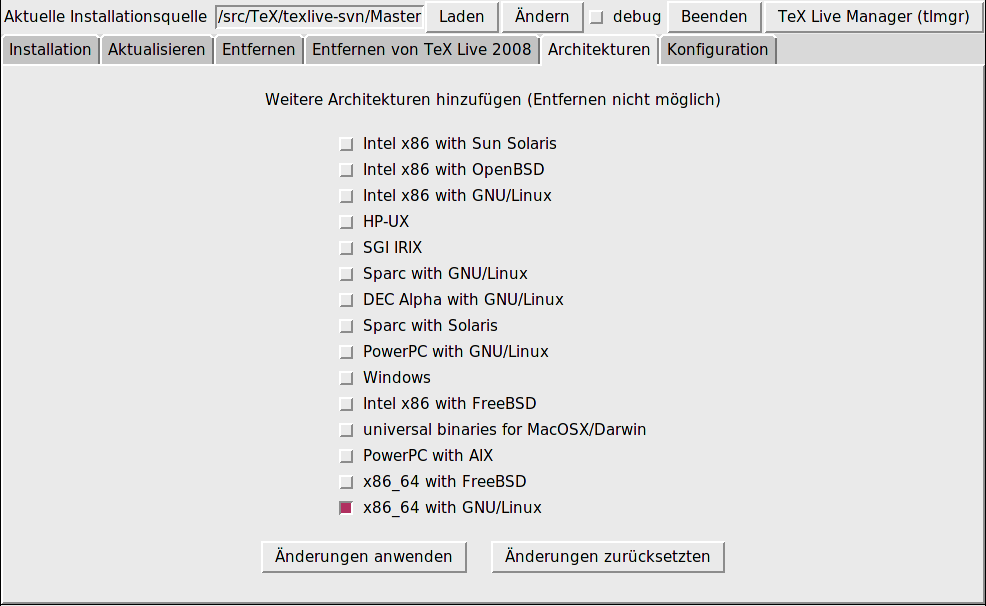
\includegraphics{tlmgrgui-arch-de.png}}
  \caption{\tlmgr\ \acro{GUI} Architekturfenster}
  \label{fig:gui:arch}
\end{figure}

Dieses Fenster listet die verfügbaren Architekturen an der aktuellen
Installationsquelle auf, und erlaubt es neue Architekturen durch
drücken des Knopfes \button{Änderungen anwenden} zu installieren.

Während das hinzufügen von Architekturen unterstützt wird, ist das
entfernen von derzeit installierten Architekturen (noch) 
nicht unterstützt. Weiters ist das gesamte Fenster unter Windows
nicht vorhanden, da Windows keine symbolischen Verweise (symlinks)
unterstützt.

\subsection{Das Konfigurationsfenster}

Dieses Fenster erlaubt es dem Benutzer sehr komfortabel diverse 
in der Datenbank gespeicherten Optionen zu überprüfen und zu ändern,
siehe Abb.~\ref{fig:gui:option}.

\begin{figure}[ht!]
  \centering
  \resizebox{0.8\columnwidth}{!}{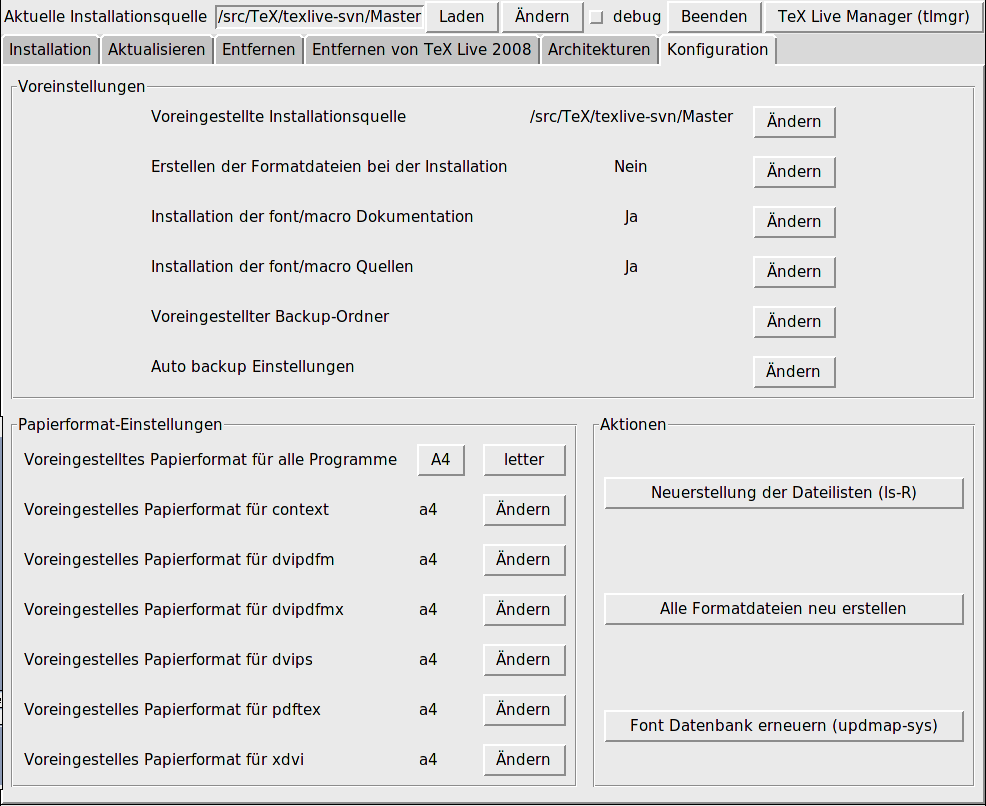
\includegraphics{tlmgrgui-options-de.png}}
  \caption{\tlmgr\ \acro{GUI} Konfigurationsfenster}
  \label{fig:gui:option}
\end{figure}

Im oberen Teil werden die in der Datenbank gespeicherten Optionen angezeigt,
und können jeweils mit dem \button{Ändern} geändert werden.

Im unteren linken Teil wird das voreingestellte Papierformat für alle
Programme angezeigt, und kann mit dem Knöpfen \button{A4} und
\button{letter} für alle Programme auf einmal geändert werden, oder
mit den Knöpfen \button{Ändern} für jedes Programm einzeln.

Im unteren rechten Teil sind einige Knöpfe die hin und wieder nützlich 
sind, nämlich um die Dateilisten (ls-R) neu zu erstellen, alle Formate
neu zu erstellen, und die Liste der Outline Schriftarten (|updmap-sys|).

\subsection{Das Logfenster}

Neben dem sich ändernden Hauptfenster gibt es ein permanentes Fenster
das die Ausgabe, die tlmgr auf die Konsole schreibt, auch in diesem
Fenster anzeigt, siehe Abb.~\ref{fig:gui:log}.

\begin{figure}[ht!]
  \centering
  \resizebox{0.8\columnwidth}{!}{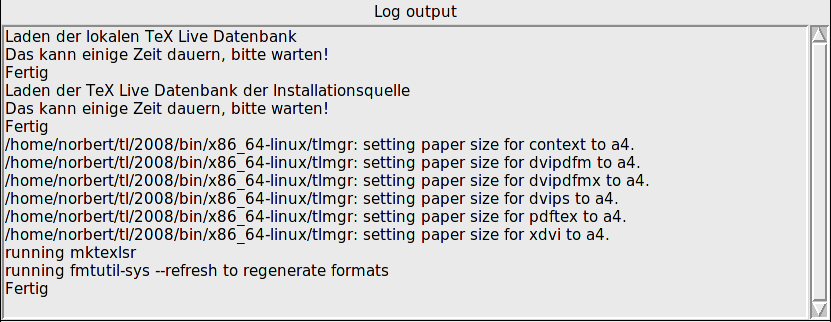
\includegraphics{tlmgrgui-log-de.png}}
  \caption{\tlmgr\ \acro{GUI} Logfenster}
  \label{fig:gui:log}
\end{figure}

\section{Was gibt es noch (neues)?}

Neben der vollkommen überarbeiteten Infrastruktur und den für Benutzer
sichtbaren Änderungen des neuen Installationsprogrammes und 
des \tlmgr wurde wie jedes Jahr alle Pakete auf den neuesten Stand 
gebracht (und auch laufend aktualisiert). Derzeit stehen circa~1400
normale Pakete wie \LaTeX\ Styles oder Fontpakete zur Verfügung, und 
zusätzlich knapp~300 andere Pakete, größtenteils Dokumentation und 
einige wenige \tl\ interne Pakete.

Das wichtigeste neue Programm ist sicher die neue \TeX-Engine Lua\TeX\
(\url{http://luatex.org}). Neben einem vollkommen neuen Grad an
Flexibilität stellt Lua\TeX\ die Scriptsprache Lua bereit, die z.\,B.\ in
|texdoc| verwendet wird.

\subsection{Windows-spezifische Eigenheiten}

Um als halbwegs komplett unter Windows zu gelten bringt jede \tl\ Installation
noch einige zusätzliche Pakete für Windows mit:
\begin{description}
\item[Perl und Ghostscript.] Da sowohl Perl als auch Ghostscript in vielen
  Programmen verwendet wird bringt \tl\ `versteckte' Kopien dieser
  Programme mit. Die \tl-Programme wissen wo sie Perl und Ghostscript
  finden können, aber diese versteckten Versionen verraten ihre Anwesenheit
  sonst nicht durch Umgebungsvariablen oder Registrierungseinträge.
  Sie sind auch kein Ersatz für eine vollständige Distribution dieser
  Programme und liefern nur die in \tl\ verwendete Funktionalität.
\item[Programme für die Kommandozeile.] 
  \tl\ installiert nun auch Portierungen von üblichen Unix-Programmen
  die zusammen mit den anderen \tl-Programmen installiert werden. Unter
  den installierten Programmen sind \cmd{gzip}, \cmd{chktex},
  \cmd{jpeg2ps}, \cmd{unzip}, \cmd{wget} und die Kommandozeilenprogramme
  der \cmd{xpdf} Suite. (Der \cmd{xpdf} Betrachter selber wird jedoch
  nicht auf Windows installiert, aber der Sumatra \acro{PDF} Betrachter
  basiert auf \cmd{xpdf}:
  \url{http://blog.kowalczyk.info/software/sumatrapdf}.)
\item[\texttt{fc-cache}] ist ein weiteres Kommandozeilenprogramm
  dass \XeTeX\ erlaubt die installierten Schriftarten effizienter
  zu handhaben.
\item[PS\_View.] Als Neuerung dieses Jahr wird PS\_View installiert,
  ein PostScript Betrachter der freie Software ist, siehe 
  Abb.~\ref{fig:psview}. Es unterstützt auch die Anzeige von \acro{PDF}
  Dateien und ist extrem schnell und hat eine Vielzahl an Funktionen.
  Bitte kontaktieren Sie uns für Vorschläge und Fehlermeldungen, dieses
  Programm ist in aktiver Entwicklung.
\item[dviout] Dieser \acro{DVI} Betrachter wurde auf der \acro{DVD} nur
  im |support| Ordner ausgeliefert, aber er wird durch Aktualisierungen
  über das Netzwerk installiert, siehe Abb.~\ref{fig:dviout}.
\end{description}

\begin{figure}[ht!]
  \centering
  \resizebox{0.8\columnwidth}{!}{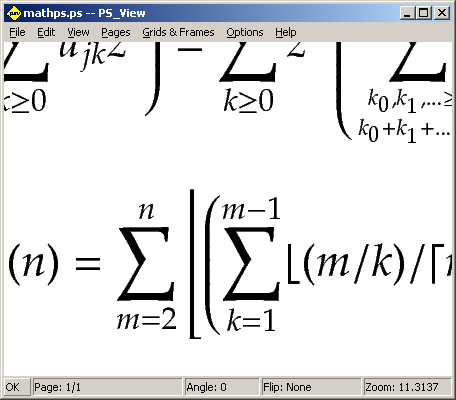
\includegraphics{psview.png}}
  \caption{PS\_View erlaubt hohe Vergrößerungen und unterstützt \acro{PDF}}
  \label{fig:psview}
\end{figure}

\begin{figure}[ht!]
  \centering
  \resizebox{0.8\columnwidth}{!}{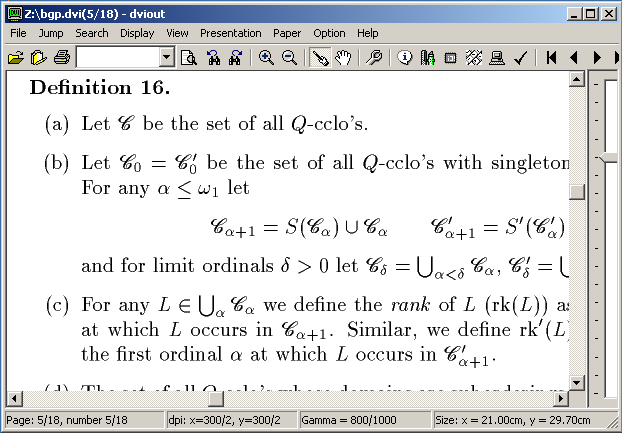
\includegraphics{dviout.png}}
  \caption{DVIout auf Windows}
  \label{fig:dviout}
\end{figure}

\section{Schlussbemerkungen und andere Informationsquellen}

Der \tlmgr\ unterliegt schneller Entwicklung, und das graphische
Frontend noch viel mehr. Wir versuchen immer mehr Funktionalität in
tlmgr einzubauen und auch in der graphischen Oberfläche abzubilden.
Bitte melden Sie jegliche Abnormalitäten an uns unter 
\url{tex-live@tug.org}.

Wie mit jedem Projekt das auf freiwillige Mitarbeit beruht leiden wir
an einem nur sehr kleinen Pool an Programmieren für die zentrale
Infrastruktur und den \tlmgr. Praktisch die gesamte Infrastruktur,
der gesamte tlmgr und das graphische Frontend wurde vom Autor mit nur 
geringen Beiträgen anderer Autoren programmiert. Jeder der Perl 
beherrscht ist herzliche eingeladen uns zu unterstützen, es gibt
lange Listen von zu erledigenden Dingen für den \tlmgr, 
ganz zu schweigen von \tl\ als Ganzes.

Wenn Sie mehr Informationen zu \tl\ suchen ist die erste Adresse
\url{http://tug.org/texlive/} und die entsprechende Dokumentationsseite
\url{http://tug.org/texlive/doc.html}.

Die Liste der Personen denen Dank gebührt ist viel zu lange um hier
inkludiert zu werden, sie ist in der online \tl\ Dokumentation, Kapitel~9
(Danksagungen) zu finden. Natürlich darf ein Name hier nicht fehlen und
das ist Karl Berry, der mit seinem unglaublichen Enthusiasmus und seiner
permanenten Unterstützung (und seiner zur gegebenen Zeit kritischen Stimme)
die Ausgabe von \tl~2008 überhaupt ermöglicht hat.

\bibliography{tlmgr-article}

%
% END OF ARTICLE
%
